%----------------------------------------
% Preamble to set up the document
%----------------------------------------
\documentclass{article}

% set up packages (you shouldn't need to touch this)
\usepackage{graphicx}  % required to insert images
\usepackage{hyperref}  % for hyperlinks
\usepackage[svgnames]{xcolor}  % to change hyperlink colors
\usepackage{tikz}
\colorlet{linkcolour}{DarkBlue}
\hypersetup{colorlinks=true, linkcolor=linkcolour, citecolor=linkcolour, urlcolor=linkcolour,}

% Margins
\topmargin=-0.45in
\evensidemargin=0in
\oddsidemargin=0in
\textwidth=6.5in
\textheight=9.0in
\headsep=0.25in

% use a sans serif font
\renewcommand{\familydefault}{\sfdefault}

%----------------------------------------
% Step 1: Edit the lecture title
%----------------------------------------
\title{
Lecture 13: Causality and Experiments \\  % Lecture title
Modeling Social Data, Spring 2019 \\   % Course title
Columbia University                    % School
}

%----------------------------------------
% Step 2: Edit your name and the date
%----------------------------------------
\author{Bailey Pierson}                     % Scribe's name
\date{April 26, 2019}                % Lecture date

\begin{document}

\maketitle


%----------------------------------------
% Step 3:
% Rename uni.tex to match your uni,
% edit the filename accordingly below,
% and put your notes in this file
%----------------------------------------
%----------------------------------------
% Write your notes here
%----------------------------------------

\section{Observational Estimates}
Picking up from last week, we know that oftentimes we are trying to compute causal effect from observed estimates, specified as follows: 

\begin{figure}[ht]
  \begin{center}
    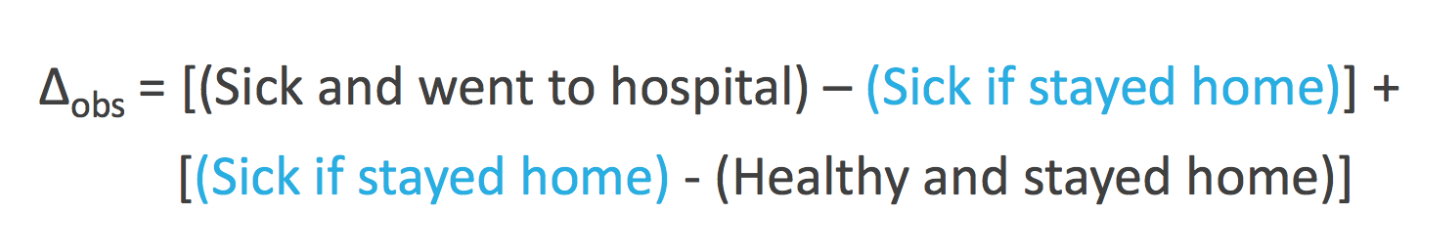
\includegraphics[width=0.5\textwidth]{figures/est.png}
  \end{center}
\end{figure}

We also briefly reviewed how selection bias comes into play here, and how simply taking the difference between observed outcomes produces a biased estimate of effect.

\begin{figure}[ht]
  \begin{center}
    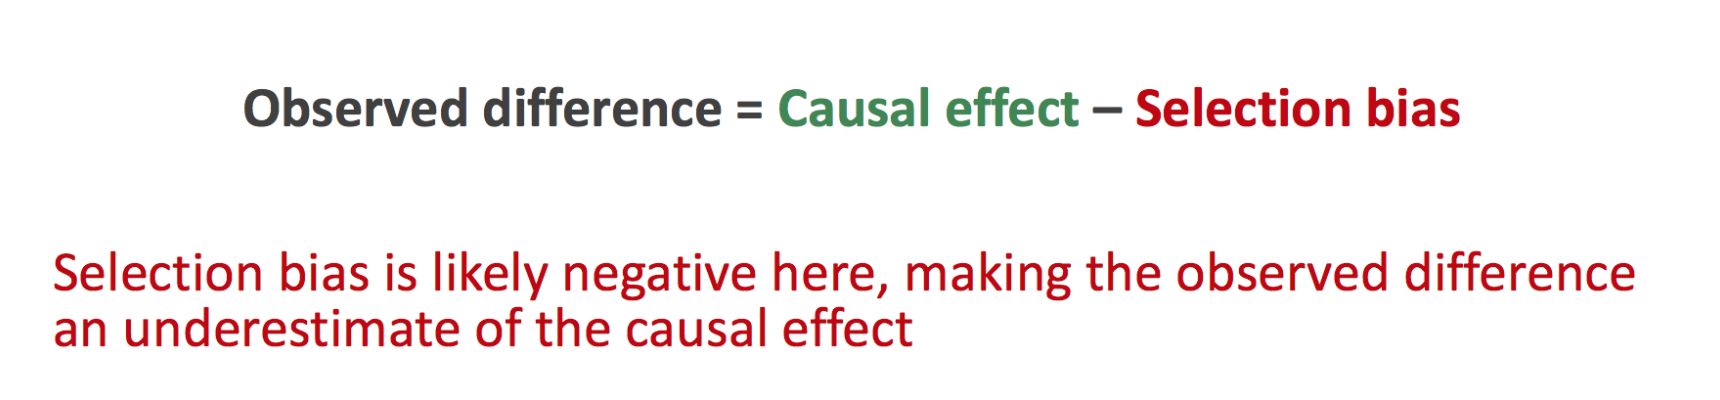
\includegraphics[width=0.5\textwidth]{figures/est2.png}
  \end{center}
\end{figure}

\section{Simpson's Paradox}
We more thoroughly covered Simpson's paradox this week. Simpson's Paradox is a phenomenon where a trend across a certain grouping of observations "disappears" or reverses when these groups are aggregated. \textbf{It is a warning against casual interpretations of causal effect, and forces us to seriously consider the underlying narrative of a causal system when making decisions on data partitioning.}

More thoroughly detailed on \href{https://en.wikipedia.org/wiki/Simpson\%27s_paradox}{Wikipedia} the UC Berkeley gender bias study is a well-known example of Simpson's Paradox. Essentially, at an aggregate level, it appeared as through admissions policy in the 1970's at Berkeley discriminated against women. 

\begin{figure}[ht]
  \begin{center}
    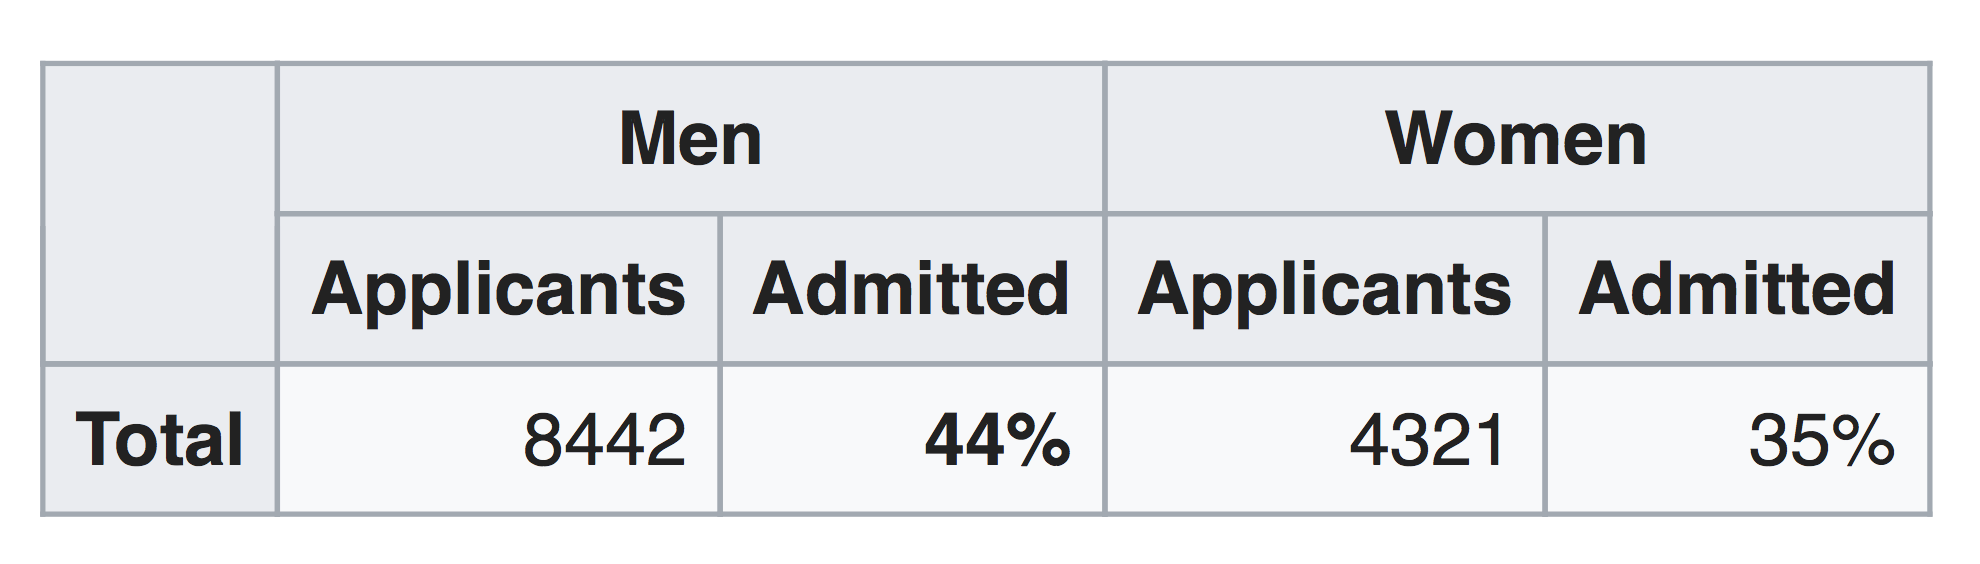
\includegraphics[width=0.5\textwidth]{figures/berk_1.png}
  \end{center}
\end{figure}

However, when dis-aggregated by department, the study concluded that women were more likely to apply to competitive departments with low rates of admission even for those qualified, while men tended to apply to less-competitive departments with high rates of admission for those qualified. 

\begin{figure}[ht]
  \begin{center}
    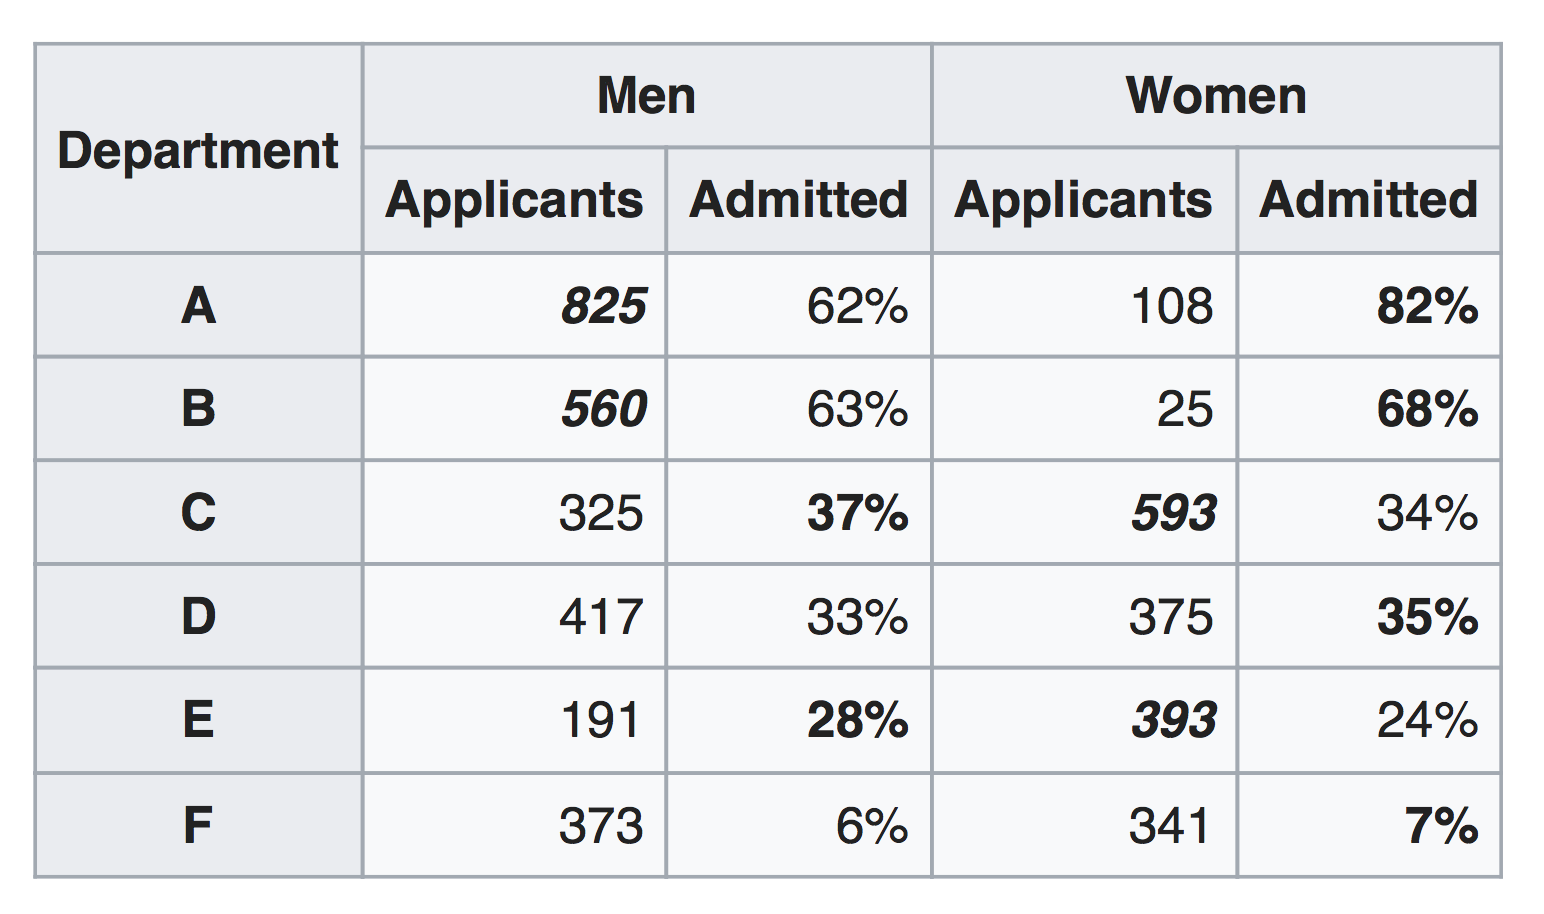
\includegraphics[width=0.5\textwidth]{figures/berk_2.png}
  \end{center}
\end{figure}


\section{Selection Bias and Causal Graphs}

It is common to represent causal systems by drawing directed graph structures, in which the direction of the edge implies that the origin node of the edge causes the destination node. The figure below shows how we might draw the relationship between college acceptance and a student having math skills and social skills. We would anticipate that having math and social skills (possibly determined via test scores or interviews) would contribute to a student's acceptance to college. 

\begin{center}
\begin{tikzpicture}[
            > = stealth, % arrow head style
            shorten > = 1pt, % don't touch arrow head to node
            auto,
            node distance = 3cm, % distance between nodes
        ]

        \tikzstyle{every state}=[
            draw = black,
            thick,
            fill = white,
            minimum size = 4mm
        ]
        
  [scale=.8,auto=center]
  \node (n1) at (7.5,5) {College Acceptance};
  \node (n2) at (5,10)  {Math Skills};
  \node (n3) at (10,10)  {Social Skills};

  \path[->] (n2)edge node {} (n1);
  \path[->] (n3) edge node {}(n1);

\end{tikzpicture}
\end{center}

Let's think about how selection bias could come into play in a situation like this. Selection bias is introduced by the selection of observations for analysis in a non-random way, resulting in a data sample that is not representative of the population we would like to analyze.  

Imagine that we condition our frequency statistics on College Acceptance, ie. we only observe students who have been accepted to college, and we want to investigate the causal effect of math vs. social skills on acceptance. Only observing accepted students, we introduce a kind of selection bias which engenders a relationship between math skills and social skills. This is because in our hypothetical college sample, there are people who are good at math and social skills, people who are bad at math  but make up for it in social skills, people who are good at math but bad at social skills, but no people who are bad at both math and social skills because they don’t even make it to college. Therefore, in our sample of accepted college students, you will find a negative correlation between math skills and social skills. This is a common problem in causal inference and again highlights how we must take into consideration all the possible relations between events in a system, lest we produce biased estimates of effects.

Note that sometimes selection bias is ok, if were are only interested in the \textbf{internal validity} of our estimates–– in this example, if we are only interested in accepted students at this specific college our finding of a negative correlation is robust and correct. However, our finding certainly does not meet standards of \textbf{external validity}, our findings do not generalize to non-accepted students.

\section{Randomization and Experiments}

As previously shown, working with observational data is difficult, and requires a lot of hand wringing in order to properly estimate causal effects. In some cases, it is possible for us to actually randomize treatment via experimental design, which allows use to directly compute the effect of treatment. However, there are some caveats to this approach.  

\begin{enumerate}
  \item Randomization often isn't feasible and/or ethical
  \item Experiments are costly in terms of time/money
  \item It is difficult to create convincing parallel worlds
  \item Effects in the lab can differ from the real world
  \item \textbf{Inevitably people deviate from their random assignments}
\end{enumerate}

There are four possible personas within a treatment assignment framework:
\begin{itemize}
  \item Compilers: Those individuals who take a treatment when assigned to a treatment groups, and do not take a treatment when assigned to a control group 
  \item Always takers: Those individuals who always take a treatment when assigned to a treatment groups AND when assigned to a control group
   \item Never takers: Those individuals who never take a treatment when assigned to a treatment groups or when assigned to a control group
  \item Defiers: Those individuals who will always do the opposite of what will tell them: will take treatment when assigned to control, or will refuse treatment when assigned to treatment (note it is rare to find true defiers in real world experiments)
\end{itemize}

\begin{figure}[ht]
  \begin{center}
    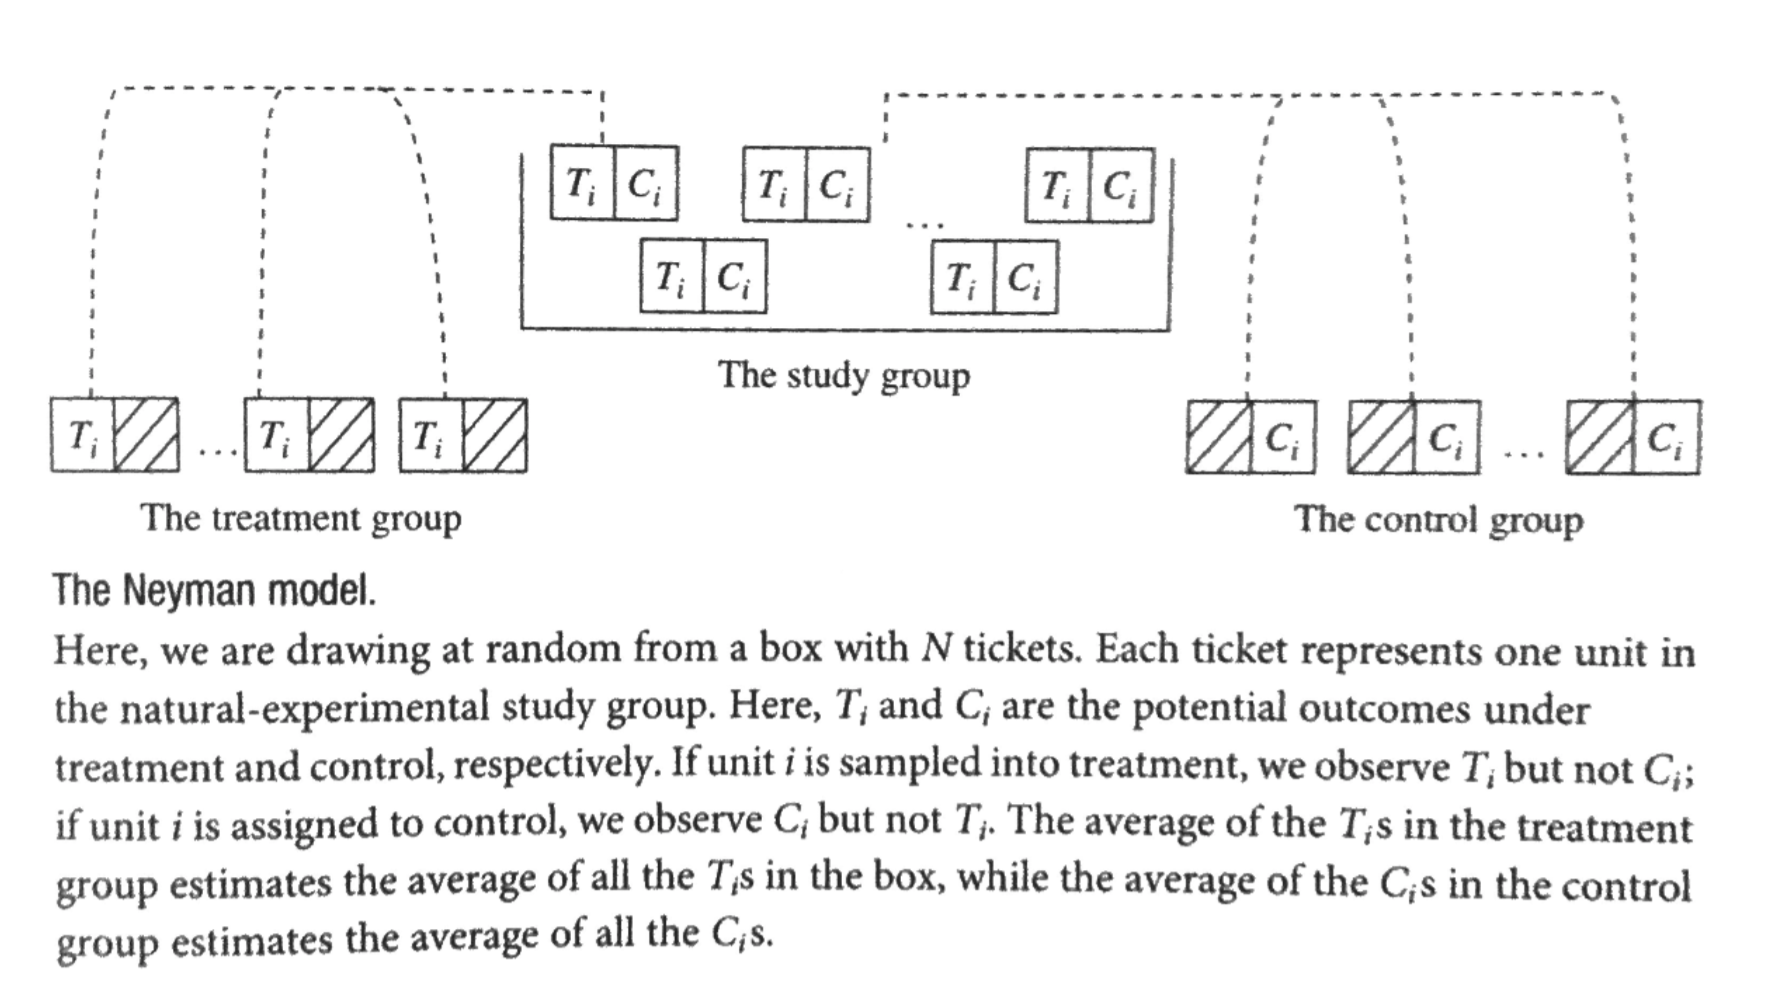
\includegraphics[width=0.5\textwidth]{figures/random.png}
  \end{center}
\end{figure}

Note that the Average Treatment Effect (often our effect of interest) can only be computed from the difference between complying individuals. 

\end{document}

%%% Local Variables:
%%% mode: latex
%%% TeX-master: t
%%% End:
